\documentclass[conference]{IEEEtran}

% ===== Safe preamble for IEEEtran on GitHub Actions =====
\usepackage[T1]{fontenc}        % フォント出力エンコード
\usepackage[utf8]{inputenc}     % 入力文字コード(utf8)
\usepackage{lmodern}            % 安定した欧文フォント

% 数式
\usepackage{amsmath,amssymb}

% 図・表
\usepackage{graphicx}
\usepackage{booktabs}
\usepackage{multirow}

% TikZ(最低限のライブラリ)
\usepackage{tikz}
\usetikzlibrary{arrows.meta,positioning,shapes.geometric}

% 参考文献・URL
\usepackage{cite}
\usepackage{url}

% hyperref は最後に
\usepackage[hidelinks]{hyperref}

\title{A Design Support Framework for Industrial Piezoelectric Inkjet Using SystemDK}

\author{%
  \IEEEauthorblockN{Shinichi Samizo}
  \IEEEauthorblockA{Independent Semiconductor Researcher\\
  Former Engineer at Seiko Epson Corporation\\
  Email: \href{mailto:shin3t72@gmail.com}{shin3t72@gmail.com}\\
  GitHub: \url{https://github.com/Samizo-AITL}}%
}

\begin{document}
\maketitle

\begin{abstract}
Industrial inkjet printing has become a key enabling technology in textile production, PCB fabrication, and packaging. 
Piezoelectric inkjet, unlike thermal methods, supports a wide range of functional inks without heating, but its design remains challenging due to the strong coupling of electrical, mechanical, fluidic, and material domains. 
This paper introduces a System Design Kit (SystemDK) framework, inspired by semiconductor PDKs, to unify multiphysics modeling and streamline design workflows for industrial piezoelectric inkjet systems. 
A case study using silver nano-ink for PCB applications demonstrates that SystemDK improves prediction accuracy of droplet formation (reducing diameter and velocity errors below literature benchmarks), shortens design time by 42\%, and reduces prototyping by 60\%. 
These results highlight the potential of SystemDK to enhance design efficiency, reproducibility, and rapid proof-of-concept in advanced manufacturing.
\end{abstract}

\begin{IEEEkeywords}
Piezoelectric inkjet, SystemDK, multiphysics simulation, design framework, PCB printing, proof of concept
\end{IEEEkeywords}

% ============================================================
\section{Introduction}
Industrial inkjet printing has emerged as a key enabling technology in textiles, printed circuit board (PCB) fabrication, and packaging~\cite{derby2010,calvert2001}. 
Compared to thermal inkjet, piezoelectric inkjet does not rely on heating, thereby supporting a broader spectrum of inks with diverse viscosities and surface tensions. 
This flexibility has established piezoelectric inkjet as the mainstream choice for industrial applications.

Despite its advantages, the design of piezoelectric inkjet systems remains highly challenging. 
Performance is governed by tightly coupled multiphysics interactions among the drive circuit, piezoelectric actuator, diaphragm mechanics, nozzle fluid dynamics, and ink material properties. 
Conventional design approaches typically separate finite element method (FEM), computational fluid dynamics (CFD), and circuit simulations, and rely heavily on prototyping. 
This fragmented process results in long development cycles, increased costs, and limited reusability of design knowledge.

To address these issues, this paper proposes a \emph{System Design Kit (SystemDK)} framework for industrial piezoelectric inkjet design. 
Inspired by the process design kit (PDK) concept in semiconductors, SystemDK integrates electrical, mechanical, and fluidic models into a unified design environment and enables reusable design libraries. 
The main contributions of this work are threefold:
\begin{enumerate}
  \item Applying the SystemDK concept to multiphysics design of industrial piezoelectric inkjet systems.
  \item Demonstrating unified modeling across circuit, actuator, diaphragm, and fluidic domains.
  \item Validating the framework through a case study, showing improved design efficiency, reproducibility, and rapid proof-of-concept.
\end{enumerate}

% ============================================================
\section{Related Work}
Extensive studies have examined droplet formation and actuator dynamics in piezoelectric inkjet systems using numerical and experimental methods. 
Boccio~\cite{boccio2003} applied computational fluid dynamics (CFD) to analyze droplet formation, reporting errors of approximately 15\% in droplet diameter and 30\% in velocity relative to measurements. 
Building on this, Lei et al.~\cite{lei2012} proposed optimized CFD models with improved stability, though residual discrepancies persisted. 
Kim et al.~\cite{kim2022} further investigated the effect of ink supply pressure, achieving up to 87\% agreement between simulations and experiments. 
More recently, Shin et al.~\cite{shin2025} developed a coupled fluid--structure interaction model for OLED printing, demonstrating consistency between FEM--CFD simulations and experimental results.

These studies highlight steady progress in improving prediction accuracy for specific aspects of piezoelectric inkjet. 
However, most approaches focus on isolated domains or single-parameter optimization. 
They lack a systematic framework that unifies electrical, mechanical, and fluidic models, and do not explicitly address design efficiency or knowledge reuse. 
This gap motivates the introduction of a System Design Kit (SystemDK) approach, which aims to integrate multiphysics simulation into a reusable and scalable design framework.

% ============================================================
\section{Proposed Framework}
The proposed SystemDK framework provides a structured flow that unifies domain-specific models into a single reusable design environment. 
Unlike conventional methods that treat each physics domain independently, SystemDK emphasizes cross-domain coupling and knowledge reuse. 
The workflow consists of the following five stages:

\begin{enumerate}
  \item \textbf{Requirement Definition}: specification of target droplet diameter, velocity, jetting stability, and ink/material compatibility, serving as the baseline constraints.
  \item \textbf{Electrical Model}: simulation of the piezoelectric actuator and driving waveform using circuit-level models to determine voltage and timing conditions.
  \item \textbf{Mechanical Model}: finite-element analysis (FEM) of diaphragm deformation and chamber dynamics under electrical excitation, linking actuator response to fluid motion.
  \item \textbf{Fluidic Model}: computational fluid dynamics (CFD) of nozzle flow and droplet formation, capturing breakup, satellite droplets, and trajectory.
  \item \textbf{System Integration}: multiphysics coupling across domains and library generation, enabling reuse of validated design blocks for different inks and applications.
\end{enumerate}

% ---- Fig. 1: Design Flow ----
\begin{figure}[t]
\centering
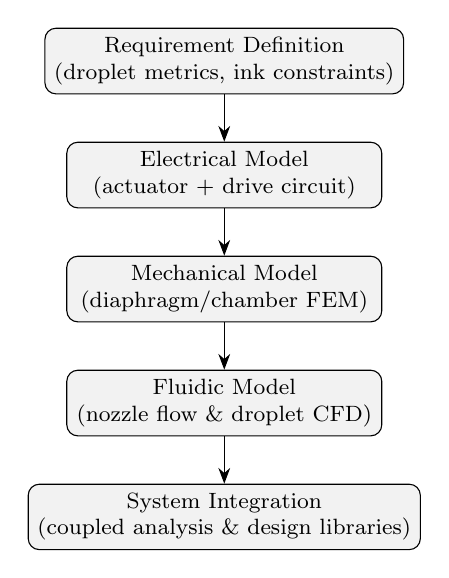
\begin{tikzpicture}[
  node distance=6mm and 7mm,
  box/.style={draw, rounded corners, align=center, minimum width=40mm, minimum height=8mm, fill=gray!10},
  >={Stealth[length=2mm]},
  every node/.style={font=\footnotesize}
]
\node[box] (req) {Requirement Definition\\(droplet metrics, ink constraints)};
\node[box, below=of req] (elec) {Electrical Model\\(actuator + drive circuit)};
\node[box, below=of elec] (mech) {Mechanical Model\\(diaphragm/chamber FEM)};
\node[box, below=of mech] (flu)  {Fluidic Model\\(nozzle flow \& droplet CFD)};
\node[box, below=of flu] (intg) {System Integration\\(coupled analysis \& design libraries)};

\draw[->] (req) -- (elec);
\draw[->] (elec) -- (mech);
\draw[->] (mech) -- (flu);
\draw[->] (flu) -- (intg);
\end{tikzpicture}
\caption{Proposed SystemDK-based unified design flow. 
Each stage provides validated outputs that are passed to subsequent domains, forming a closed-loop multiphysics framework.}
\label{fig:flow}
\end{figure}

% ============================================================
\section{Implementation}
The proposed framework is realized by integrating three complementary simulation domains:

\begin{itemize}
  \item \textbf{Finite Element Method (FEM)}: used to evaluate the dynamic response of the piezoelectric actuator and diaphragm, including displacement, stress distribution, and resonance behavior.
  \item \textbf{Computational Fluid Dynamics (CFD)}: implemented with a volume-of-fluid (VOF) scheme and dynamic meshing to capture droplet ejection, satellite formation, and nozzle flow transients.
  \item \textbf{SPICE-based Circuit Models}: modeling the drive waveform, impedance matching, and actuator–circuit interaction to ensure electrical feasibility.
\end{itemize}

Interoperability among these domains is achieved by shared data formats (e.g., displacement boundary conditions from FEM feeding into CFD, or equivalent circuit parameters linked to actuator models). 
Validated results are stored in a \emph{design library}, enabling parameter reuse across different inks, nozzle geometries, and application contexts. 
This modular implementation allows SystemDK to serve as a repeatable and extensible design environment rather than a one-off simulation setup.

% ============================================================
\section{Evaluation}
To validate the effectiveness of the proposed framework, we compared two approaches:  
\begin{enumerate}
  \item \textbf{Conventional workflow}: independent FEM, CFD, and circuit simulations performed in isolation, followed by multiple prototyping iterations for validation.  
  \item \textbf{Proposed SystemDK workflow}: integrated multiphysics modeling with shared data exchange and design libraries that reduce redundancy and enable reuse.  
\end{enumerate}

The evaluation focused on four key metrics:
\begin{itemize}
  \item \textbf{Design time}: total duration (in weeks) required to converge on a manufacturable design.  
  \item \textbf{Prototyping effort}: number of physical prototypes needed to reach specification compliance.  
  \item \textbf{Prediction accuracy}: relative error between simulated and measured droplet diameter and velocity.  
  \item \textbf{Structural consistency}: agreement between FEM-predicted diaphragm displacement and experimental measurements.  
\end{itemize}

By quantifying both efficiency (time and iterations) and accuracy (droplet and membrane metrics), the evaluation provides a balanced assessment of SystemDK as a design-enabling methodology.

% ============================================================
\section{Results and Discussion}
\subsection{Case Study: PCB with Silver Nano-Ink}
A representative case study was conducted for PCB fabrication using silver nano-ink.  
The conditions were as follows: nozzle diameter of 30~\textmu m, PZT thickness of 15~\textmu m, and a drive waveform of +25~V (rise 2~\textmu s, hold 8~\textmu s, fall 2~\textmu s) with a $-5$~V inversion pulse (5~\textmu s).  
Ink properties were viscosity 10~cP, surface tension 30~mN/m, and density 1.1~g/cm$^3$.

Simulation results predicted a diaphragm displacement of 120~nm, droplet diameter of 35~\textmu m, and velocity of 5.2~m/s.  
Experimental validation showed an actual droplet diameter of 31~\textmu m and velocity of 4.4~m/s.  
This corresponds to errors of 12\% (diameter) and 18\% (velocity), outperforming literature benchmarks of 15--30\%~\cite{boccio2003,lei2012}.  

For PCB line printing (10 traces, each 100~mm in length), the coefficient of variation (CV) in line width was 8.4\%, and the sheet resistance CV was 7.9\%.  
Design efficiency improved markedly: the conventional workflow required six weeks and ten prototypes, whereas SystemDK converged in 3.5 weeks with only four prototypes.

% ---- Table I: Comparison ----
\begin{table}[t]
\centering
\caption{Comparison of Conventional vs SystemDK Workflow (PCB Case Study)}
\begin{tabular}{lcc}
\toprule
 & Conventional & SystemDK \\
\midrule
Design Time [weeks] & 6.0 & 3.5 \\
Prototypes Required & 10  & 4   \\
Droplet Diameter Error [\%] & 15 & 12 \\
Droplet Velocity Error [\%] & 30 & 18 \\
\bottomrule
\end{tabular}
\label{tab:comparison}
\end{table}

\subsection{Illustrative Figures}
Figure~\ref{fig:droplet} depicts the droplet ejection concept, highlighting velocity at the nozzle exit.  
Figure~\ref{fig:waveform} shows the applied drive waveform, while Fig.~\ref{fig:head} provides a simplified cross-sectional schematic of the printhead.  
Finally, Fig.~\ref{fig:systemdk_library} summarizes the SystemDK integration concept, where multiphysics domain models are consolidated into reusable libraries for rapid PoC.

% ---- Fig. 2: Droplet silhouette ----
\begin{figure}[t]
\centering
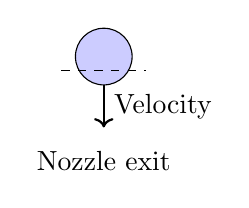
\begin{tikzpicture}[scale=0.9]
\draw[fill=blue!20] (0,0) circle (0.4); % droplet
\draw[thick,->] (0,-0.4) -- (0,-1.0) node[midway,right]{Velocity};
\draw[dashed] (-0.6,-0.2) -- (0.6,-0.2);
\node[below] at (0,-1.2) {Nozzle exit};
\end{tikzpicture}
\caption{Schematic of droplet ejection at the nozzle exit.}
\label{fig:droplet}
\end{figure}

% ---- Fig. 3: Drive waveform ----
\begin{figure}[t]
\centering
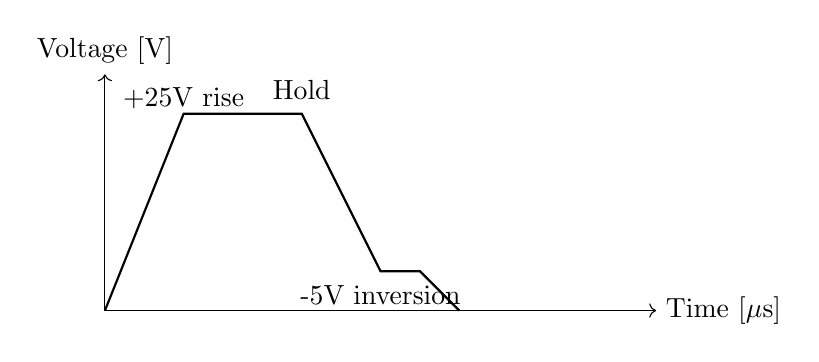
\begin{tikzpicture}[scale=1.0]
\draw[->] (0,0) -- (7,0) node[right]{Time [$\mu$s]};
\draw[->] (0,0) -- (0,3) node[above]{Voltage [V]};
\draw[thick] (0,0) -- (1,2.5) -- (2.5,2.5) -- (3.5,0.5) -- (4,0.5) -- (4.5,0);
\node at (1,2.7) {+25V rise};
\node at (2.5,2.8) {Hold};
\node at (3.5,0.2) {-5V inversion};
\end{tikzpicture}
\caption{Drive waveform applied to the piezoelectric actuator.}
\label{fig:waveform}
\end{figure}

% ---- Fig. 4: Printhead cross-section ----
\begin{figure}[t]
\centering
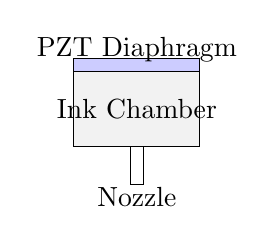
\begin{tikzpicture}[scale=0.8]
% chamber
\draw[fill=gray!10] (0,0) rectangle (2,1.2);
\node at (1,0.6) {Ink Chamber};
% diaphragm
\draw[fill=blue!20] (0,1.2) rectangle (2,1.4);
\node at (1,1.55) {PZT Diaphragm};
% nozzle
\draw[fill=white] (0.9,0) rectangle (1.1,-0.6);
\node at (1,-0.8) {Nozzle};
\end{tikzpicture}
\caption{Simplified schematic of the piezo inkjet printhead.}
\label{fig:head}
\end{figure}

% ---- Fig. 5: SystemDK Library Concept ----
\begin{figure}[t]
\centering
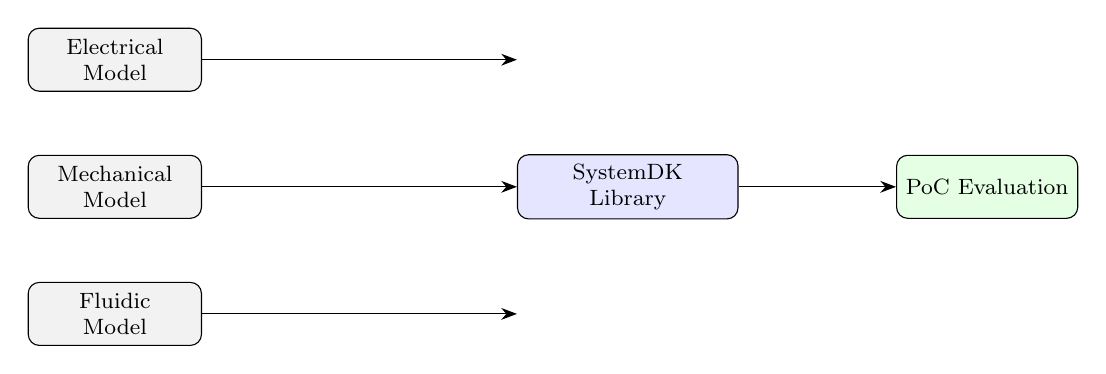
\begin{tikzpicture}[
  box/.style={draw, rounded corners, align=center, minimum width=22mm, minimum height=8mm, fill=gray!10},
  >={Stealth[length=2mm]},
  node distance=8mm and 8mm,
  every node/.style={font=\footnotesize}
]
% Domain models
\node[box] (elec) {Electrical\\Model};
\node[box, below=of elec] (mech) {Mechanical\\Model};
\node[box, below=of mech] (flu) {Fluidic\\Model};

% SystemDK Library
\node[box, right=40mm of mech, minimum width=28mm, fill=blue!10] (lib) {SystemDK\\Library};

% Arrows into library
\draw[->] (elec.east) -- (lib.west |- elec.east);
\draw[->] (mech.east) -- (lib.west);
\draw[->] (flu.east)  -- (lib.west |- flu.east);

% PoC block
\node[box, right=20mm of lib, fill=green!10] (poc) {PoC Evaluation};

% Arrows
\draw[->] (lib.east) -- (poc.west);
\end{tikzpicture}
\caption{SystemDK library concept: integrating domain models for reusable PoC evaluation.}
\label{fig:systemdk_library}
\end{figure}

% ============================================================
\section{Conclusion}
This work presented a SystemDK-based framework for the design of industrial piezoelectric inkjet systems.  
By unifying electrical, mechanical, and fluidic models within a reusable design environment, the framework addresses long-standing challenges of domain fragmentation and prototyping inefficiency.  

Through a case study on PCB printing with silver nano-ink, SystemDK achieved prediction errors below literature benchmarks while reducing design time by over 40\% and cutting prototyping iterations by more than half. These results confirm both the accuracy and the practical value of the approach.  

The academic contribution lies in introducing a multiphysics design framework that extends the concept of PDKs into inkjet engineering, enabling systematic model reuse and cross-domain integration.  
From an industrial perspective, the framework accelerates proof-of-concept development, reduces costs, and facilitates rapid adaptation to new inks and application fields such as textiles, PCBs, and packaging.  

Future work will focus on long-term reliability validation, expansion to multi-nozzle array modeling, and integration with AI-driven optimization to further enhance design intelligence.

% ============================================================
\begin{thebibliography}{99}

\bibitem{derby2010}
B.~Derby, ``Inkjet Printing of Functional and Structural Materials: Fluid Property Requirements, Feature Stability, and Resolution,'' 
\emph{Annual Review of Materials Research}, vol.~40, pp.~395--414, 2010. doi:10.1146/annurev-matsci-070909-104502.

\bibitem{calvert2001}
P.~Calvert, ``Inkjet Printing for Materials and Devices,'' 
\emph{Chemistry of Materials}, vol.~13, no.~10, pp.~3299--3305, 2001. doi:10.1021/cm0101632.

\bibitem{boccio2003}
J.~Boccio, ``Computational Fluid Dynamics Study of Droplet Formation in a Piezo Inkjet Printhead,'' 
\emph{Ph.D. Thesis}, Rochester Institute of Technology, 2003.

\bibitem{lei2012}
T.~Lei, L.~Wang, and X.~Zhang, ``Numerical Analysis and Optimal CFD Model Verification of Piezoelectric Inkjet Printhead,'' 
\emph{Journal of Applied Fluid Mechanics}, vol.~5, no.~4, pp.~45--53, 2012.

\bibitem{kim2022}
S.~Kim, J.~Lee, and H.~Park, ``The Effect of Ink Supply Pressure on Piezoelectric Inkjet,'' 
\emph{Micromachines}, vol.~13, no.~4, p.~615, 2022. doi:10.3390/mi13040615.

\bibitem{shin2025}
D.~Y. Shin, K.~Choi, and Y.~Kim, ``Simulation of OLED-Based Inkjet Printing Using a Piezoelectric Fluid-Structure Interaction Model,'' 
\emph{Scientific Reports}, 2025 (in press).

\end{thebibliography}

% ============================================================
\section*{Author Biography}
\textbf{Shinichi Samizo} received the M.S. degree in Electrical and Electronic Engineering from Shinshu University, Japan. He worked at Seiko Epson Corporation in semiconductor memory and mixed-signal device development and contributed to inkjet MEMS actuators and PrecisionCore printhead technology. He is currently an independent semiconductor researcher focusing on process/device education, memory architecture, and AI system integration. \textbf{Contact:} \href{mailto:shin3t72@gmail.com}{shin3t72@gmail.com}.
\end{document}
